\documentclass[11pt]{article}

\usepackage[english]{babel}
\usepackage[utf8]{inputenc}
\usepackage{kpfonts}
\usepackage[left=2.75cm, right=2.75cm, top=2.8cm, bottom=3cm]{geometry}
\usepackage{titling}
\usepackage{graphicx}
\usepackage{hyperref}
\usepackage{tikz}
\usepackage{amsmath}
\usepackage{algorithm}
\usepackage{algpseudocode}
\usepackage{wrapfig}

\graphicspath{{ims/}}

\newcommand{\N}{\mathbb{N}}
\newcommand{\Z}{\mathbb{Z}}
\newcommand{\R}{\mathbb{R}}

%%%%%%%%%%%% Title Part %%%%%%%%%%%%
\pretitle{
	\begin{center}
	\includegraphics[width=3.5cm]{logo_ens_lyon.pdf}
	\hspace{5cm}
	
\includegraphics[width=4.7cm]{logo_tu_delft.png}
	\LARGE
}
\title{
	\rule{\linewidth}{0.4mm}
	\textbf{Perspective Check in Paintings} \\
	\textit{M1 Internship}
	\rule{\linewidth}{0.6mm} \vspace{-10mm}
}
\author{
	Yoann Coudert--Osmont \\[1.5mm]
	\textit{Supervised by} \\
	Elmar Eisemann \qquad Ricardo Marroqium \\[2mm]
}
\date{May - July 2019}
%%%%%%%%%%%%%%%%%%%%%%%%%%%%%%%%%%%%

\begin{document}
	\maketitle
	
	\section*{Introduction}
	
	\begin{figure}
		\centering
		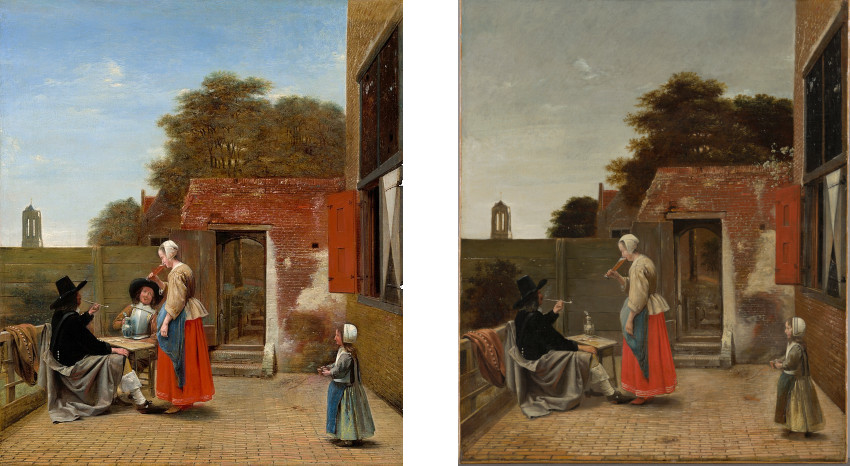
\includegraphics[scale=1.25]{paintings_pair.jpg}
		\caption{A pair of similar paintings}
		\label{im:pair}
	\end{figure}

	In a Delft museum, paintings by Pieter de Hooch are on display. It is quite easy to notice that some pairs of paintings are very similar (e.g. \figurename \ref{im:pair}). One hypothesis that would explain this strangeness is the possibility that another painter copied Pieter de Hooch's paintings. Looking at the pairs in more detail, we can notice that quite often one painting respects the rules of perspective well and the other does not respect them. This gives credibility to the hypothesis of the existence of another painter. But the human tends to be biased to check that in each pair, one painting respects the rules of perspective and the other does not. Then comes the need to create a tool to check whether the perspective is respected in a painting with as little human intervention as possible. The goal of this internship was therefore to create a graphical interface to verify the perspective in a painting with as much automation as possible. \\
	Tools already exist to find lines in an image. The most common and the one I used is the Hough transform \cite{hough}. I will describe the algorithms used to create my interface in this report. In most paintings there is a tiled floor and it is mainly the lines of the tiles that I studied. The development of a graphical user interface with minimal user control was necessary because there is no guarantee that a fully automated program will do exactly what we want. Part of the internship was used to learn how to make a graphical interface with Qt and to design an interface that is easily usable. But I'm not going to describe how this interface works, I'll just give some implemented features inside this report.

	\vspace{3cm}
	\begin{center}
		\tableofcontents
	\end{center}
	
	\newpage
	
	\section{Reminders on the rules of perspective}
	
	The main rule of perspective is that when you make a drawing, the parallel lines must all cross at the same point. We call this point a vanishing point. In addition, all vanishing points must be on the same line. This line is the vanishing line and corresponds to the horizon.
	
	\begin{figure}[h]
		\centering
		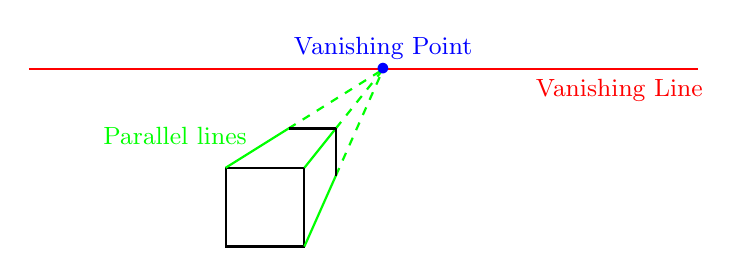
\begin{tikzpicture}[thick]
			\draw[] (0, 0) -- (1, 0) -- (1, 1) -- (0, 1) -- cycle;
			\draw[red] (-2.5, 2.25) -- (6, 2.25);
			\draw[green] (0, 1) -- (0.8, 1.5);
			\draw[green, dashed] (0.8, 1.5) -- (2, 2.25);
			\draw[green] (1, 1) -- (1.4, 1.5);
			\draw[green, dashed] (1.4, 1.5) -- (2, 2.25);
			\draw (0.8, 1.5) -- (1.4, 1.5);
			\draw[green] (1, 0) -- (1.4, 0.9);
			\draw[green, dashed] (1.4, 0.9) -- (2, 2.25);
			\draw (1.4, 0.9) -- (1.4, 1.5);
			
			\node[blue] (VP) at (2, 2.25) {$\bullet$};
			\node[above, blue] at (2, 2.25) {\small Vanishing Point};
			\node[below, red] at (5, 2.25) {\small Vanishing Line};
			\node[left, green] at (0.4, 1.4) {\small Parallel lines};
		\end{tikzpicture}
		\vspace{-2mm}
		\caption{Illustration of the perspective rules}
	\end{figure}
	\vspace{-2mm}

	\subsection{Special case of a tiled floor}
	
	This subsection will be useful for the last section of this report. There are two interesting equations to record about tiled floors linking tile lines with their diagonals. Indeed I will try to build a new painting that perfectly respects the perspective. But to do this, it is necessary to know the properties that the vanishing points of a tiled floor must respect.
	
	\begin{figure}[h]
		\centering
		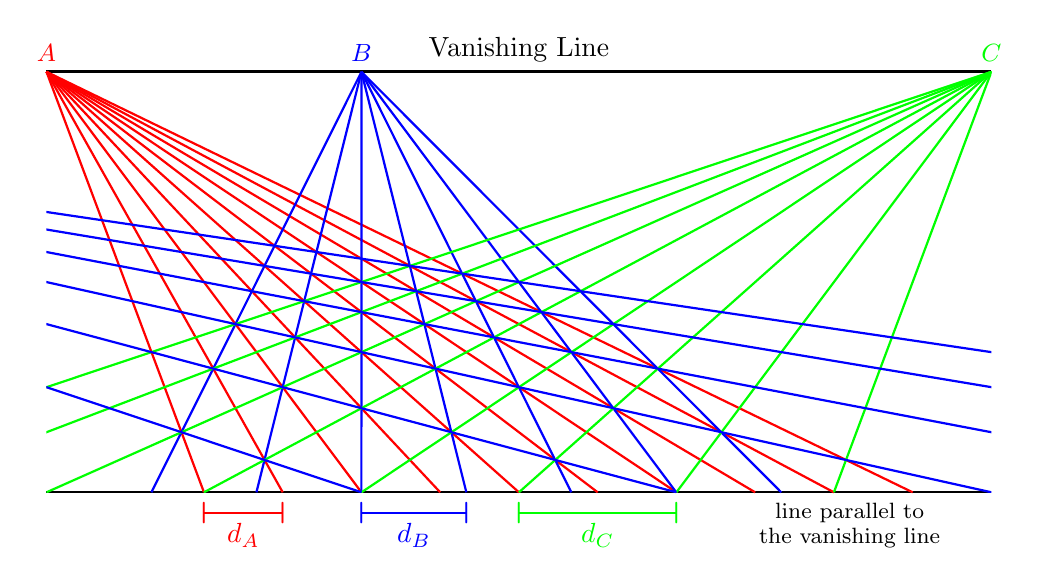
\begin{tikzpicture}[thick, yscale=0.89]
		\draw[very thick] (0, 6) -- (12, 6);
		\draw[semithick] (0, 0) -- (12, 0);
		\node[above] at (6, 6) {Vanishing Line};
		\node[above, red] at (0, 6) {\small $A$};
		\node[above, blue] at (4, 6) {\small $B$};
		\node[above, green] at (12, 6) {\small $C$};
		
		\foreach \i in {2, ..., 11} \draw[red] (0, 6) -- (\i, 0);
		\foreach \i in {1.333, 2.666, ..., 9.333} \draw[blue] (4, 6) -- (\i, 0);
		
		\draw[red] (2, -0.3) node {\texttt{|}} -- node[below] {$d_A$} (3, -0.3) node {\texttt{|}};
		\draw[blue] (4, -0.3) node {\texttt{|}} -- node[below] {$d_B$} (5.333, -0.3) node {\texttt{|}};
		\draw[green] (6, -0.3) node {\texttt{|}} -- node[below] {$d_C$} (8, -0.3) node {\texttt{|}};
		
		\node[below, align=center] at (10.2, 0)
			{\footnotesize line parallel to \\[-1mm]
			\footnotesize the vanishing line};
		
		\clip (0, 0) rectangle (12, 6);
		\foreach \i in {-4, -2, ..., 10} \draw[green] (12, 6) -- (\i, 0);
		\foreach \i in {4, 8, ..., 24} \draw[blue] (-12, 6) -- (\i, 0);
		\end{tikzpicture}
		\vspace{-3mm}
		\caption{Tiled floor in perspective}
		\label{im:tiledfloor}
	\end{figure}

	In the \figurename \ref{im:tiledfloor}, blue lines represent a tiled floor in perspective. We will always assume that tiles are squares. Then all the parallel lines are equally spaced. In perspective, this implies that if a line parallel to the vanishing line is drawn, then the tile lines intersect with it at regular intervals. We write these intervals $\color{blue} d_B$ for the depth lines, and $\color{red} d_A$ and $\color{green} d_C$ for the diagonals. $\color{red} A$, $\color{blue} B$ and $\color{green} C$ are the vanishing points located on the vanishing line (note that here the vanishing line is horizontal but it may not be). Finally here are the two equations respected by such a tiled floor:
	
	\begin{center}
		\begin{minipage}{0.3\linewidth}
			\begin{equation}
			\label{eq:B}
			{\color{blue} B} = \dfrac{{\color{green} d_C} {\color{red} A} + {\color{red} d_A} {\color{green} C}}{{\color{red} d_A} + {\color{green} d_C}}
			\end{equation}
		\end{minipage}
		\begin{minipage}{0.3\linewidth}
			\begin{equation}
			\label{eq:dB}
			{\color{blue} d_B} = 2 \dfrac{{\color{red} d_A} {\color{green} d_C}}{{\color{red} d_A} + {\color{green} d_C}}
			\end{equation}
		\end{minipage}
	\end{center}
	
	\section{Description of the algorithm}
	
	% Need to talk about what I tried before hough transform (PCA on connex components)

	\subsection{General description}
	\label{s:general}
	
	\paragraph{}
	Finding lines in an image can be broken down into several steps. For my part, I divided this task into four main steps. First I change the color space to switch from RGB space to CIE Lab space \cite{cielab}. Then I eliminate the noise and smooth the image while keeping the areas with high gradient. In the third step I compute in each pixel of the image the direction and amplitude of the gradient. I leave some user control over the value of some thresholds used in this step. In addition, the user has the possibility to erase certain parts of the gradient that are not interesting to study perspective. Finally, the last step consists in applying the Hough transform to the gradient. The local maxima of this transformation then give us the lines contained in the image.
	
	Once the user has obtained the lines of the image he has the possibility to make groups in order to calculate the vanishing points, the vanishing line but also to calculate the diagonals of a tiled floor as we could see in the previous part. Once the user has finished this part he can judge if the perspective is well respected.
	
	\subsection{Color Space}
	
	\paragraph{}
	At the beginning of my experiments I did not make any color space changes. The gradient of the image was calculated in the RGB space well known to all. In this space the colors are represented by three bytes, representing respectively the intensity of red, green and blue in the color. Unfortunately for some paintings, the amplitude of the gradient obtained did not necessarily match what I observed with the naked eye. My algorithm could return a high gradient where I could only see a slight color change and return a low gradient where I could see a boundary between two distinct colors. One of the concerns of RGB space, for example, is that it does not take into account the fact that the human eye is less sensitive to the color blue than to the color green.
	
	\paragraph{}
	The CIELAB space \cite{cielab} allows you to correct this problem. Indeed, the Euclidean distance in this space corresponds well to the difference in color that a human observes with his eyes. It is a space more in line with human vision. The three coordinates of CIELAB represent the lightness of the color ($L^* = 0$ yields black and $L^* = 100$ indicates diffuse white), its position between red/magenta and green ($a^*$, negative values indicate green while positive values indicate magenta) and its position between yellow and blue ($b^*$, negative values indicate blue and positive values indicate yellow). Thus the difference between two colors $(L_1^*, a_1^*, b_1^*)$ and $(L_2^*, a_2^*, b_2^*)$ is given by the Euclidean distance:
	$$ \Delta E = \sqrt{(L_1^* - L_2^*)^2 + (a_1^* - a_2^*)^2 + (b_1^* - b_2^*)^2} $$
	
	\paragraph{}
	I will not give the formulas for switching from RGB to CIELAB, but I can give the intermediate steps. There is first a non-linear transformation from RBG to sRGB then a linear transformation to the XYZ space and finally a non-linear transformation from XYZ to CIELAB. Once this change of space was implemented, the results on some paints improved considerably.
	
	\subsection{Smoothing}
	
	\paragraph{}
	Smoothing is often important in image processing because it allows noise to disappear. There are many filters known to perform smoothing. There is for example the median filter which replaces each pixel by the median value on a neighborhood, or the very used Gaussian filter which has the particularity to be applied with a low complexity thanks to a Fourrier transform. The Gaussian filter performs a weighted average of the neighboring pixels. This weighting is done using a Gaussian with a standard deviation $\sigma$. Averages are taken individually on each component of the color space. If we consider an image $I : \N \times \N \rightarrow \R$ which associates real values to integer coordinates, then applying a Gaussian filter of standard deviation $\sigma$ gives the following image $I'$:
	$$ I'(z) = \dfrac{1}{W} \sum_{z' \in \Omega_{z}} I(z') \exp \left( - \dfrac{\| z - z'\|^2}{2 \sigma^2} \right) $$
	Where $\Omega_{z}$ is a window around $z \in \N^2$ and $W = \sum_{z' \in \Omega_{z}} \exp \left( - \frac{\| z - z'\|^2}{2 \sigma^2} \right)$ is a factor of normalization. Since it is a convolution product, this can be computed in the Fourier space with a point-wise product. That's the big advantage of this filter. The problem is that it could erase borders that would be useful for finding the lines in the image.
	
	\paragraph{}
	One solution to overcome these important edge disappearances is to use a bilateral filter \cite{bil}. This filter is defined using two functions $f: \N^2 \times \N^2 \rightarrow \R$ and $g: \R \times \R \rightarrow \R$ and gives the following image:
	$$ I'(z) = \dfrac{1}{W} \sum_{z' \in \Omega_{z}} I(z) \, f(z, z') \, g \left( I(z), I(z') \right) $$
	Where $\Omega_{z}$ is still a window around $z$ and $W = \sum_{z' \in \Omega_{z}} f(z, z') g(I(z), I(z'))$. Thanks to the $g$ function, not only the position of the other pixels is taken into account, but also the value of these pixels. The idea we can then have is to use this $g$ function to ignore pixels that have a too different color in order not to smooth the borders between two different colors. Taking two Gaussian functions for f and g is then common practice and that is the choice I made:
	$$ f(z, z') = \exp \left( - \dfrac{\| z - z'\|^2}{2 \sigma_f^2} \right) \qquad g(u, u') = \exp \left( - \dfrac{\| u - u'\|^2}{2 \sigma_g^2} \right) $$
	The two standard deviations ($\sigma_f$ and $\sigma_g$) and the size of the neighborhood are automatically calculated according to certain image characteristics.
	
	\begin{figure}[h]
		\centering
		\begin{tikzpicture}
			\node at (0, 0.9) {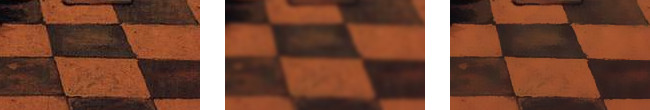
\includegraphics[width=10cm]{smoothing.jpg}};
			\node[below] at (0, 0) {Gaussian filter};
			\node[below] at (-3.45, 0) {Original image};
			\node[below] at (3.45, 0) {Bilateral filter};
		\end{tikzpicture}
		\vspace{-1mm}
		\caption{Comparison of smoothing filters}
		\label{im:smooths}
	\end{figure}
	\vspace{-1mm}

	\paragraph{}
	It can be seen in the \figurename \ref{im:smooths} that the bilateral filter keeps the edges clean between the tiles and that the noise inside the tiles is erased. This filter therefore does exactly what we want it to do, unlike the Gaussian filter which smooths the edges between the tiles and therefore makes it difficult to accurately locate the edges. On the other hand because of the function $g$, the filter is not a convolution product and it is therefore no longer possible to go through the Fourier transform in order to calculate the results in a fast way. That's the only downside of this filter. To compensate for this calculation time which can be long and even to simplify the steps that will follow, I leave the user the possibility to select with a lasso the interesting area to study in the painting (\figurename \ref{im:cut}).
	
	\begin{figure}[h]
		\centering
		\begin{tikzpicture}
		\node (a) at (0, 0) {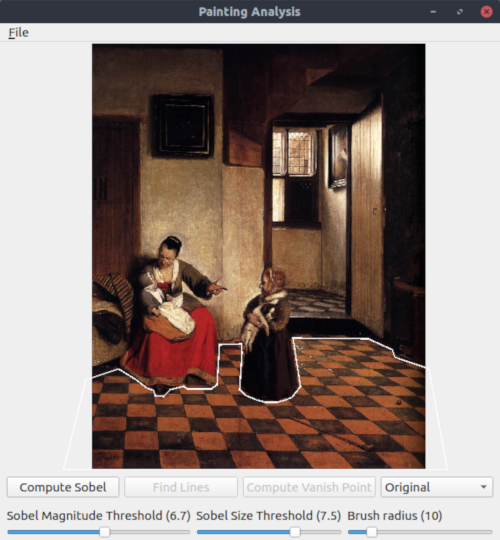
\includegraphics[scale=1]{zone_select.png}};
		\node (b) at (8, 0) {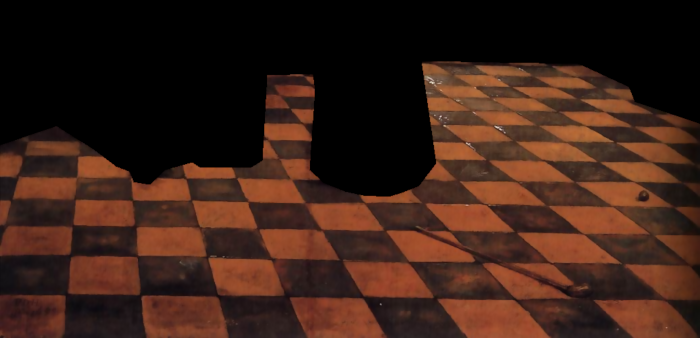
\includegraphics[scale=1.2]{bilateral.png}};
		\draw[->, ultra thick] (a) -- node[above, align=center]
			{\footnotesize Cut the image \\[-1mm]
				\footnotesize and apply \\[-1mm]
				\footnotesize bilateral filter} (b);
		\end{tikzpicture}
		\vspace{-1mm}
		\caption{The user has the possibility to select the interesting zone.}
		\label{im:cut}
	\end{figure}
	
	\subsection{Gradient}
	
	\paragraph{}
	To compute the gradient of the image, I used a Sobel filter of size $3$ by $3$. This filter calculates the amplitude of the gradient along the x-axis and the y-axis and then deduces the gradient norm and direction from it. This is done for each $C$ component of the CIELAB space. I denote by $\ast$ the convolution product. We then have:
	$$ G_{C, x} = \begin{bmatrix} -3 & 0 & 3 \\ -10 & 0 & 10 \\ -3 & 0 & 3 \end{bmatrix} \ast C
		\qquad G_{C, y} = \begin{bmatrix} -3 & -10 & -3 \\ 0 & 0 & 0 \\ 3 & 10 & 3 \end{bmatrix} \ast C
	$$
	Where $G_{C, x}$ and $G_{C, y}$ are are respectively the discrete horizontal and vertical gradients of the component $C$. We can then compute the norm of the gradient in this component:
	$$ G_C = \sqrt{G_{C, x}^2 + G_{C, y}^2} $$
	As only the direction of the gradient and not the orientation of the gradient interests us, we want to compute the angle of the gradient modulo $\pi$ instead of $2 \pi$. We then defines $(G_{C, x}', \, G_{C, y}')$ equal to $(G_{C, x}, \, G_{C, y})$ if $G_{C, x} \geqslant 0$ or to $(-G_{C, x}, \, -G_{C, y})$ otherwise. Finally, the norm $G$ and the angle $\Theta$ of the gradient are obtained as follows:
	$$ G = \sqrt{G_{L^*} + G_{a^*} + G_{b^*}} \qquad \Theta = \arg \left( G_{L^*} G_{L^*, x}' + G_{a^*} G_{a^*, x}' + G_{b^*} G_{b^*, x}' + i \left( G_{L^*} G_{L^*, y}' + G_{a^*} G_{a^*, y}' + G_{b^*} G_{b^*, y}' \right) \right)$$
	
	\begin{figure}[h]
		\centering
		\begin{tikzpicture}
		\node at (0, 0) {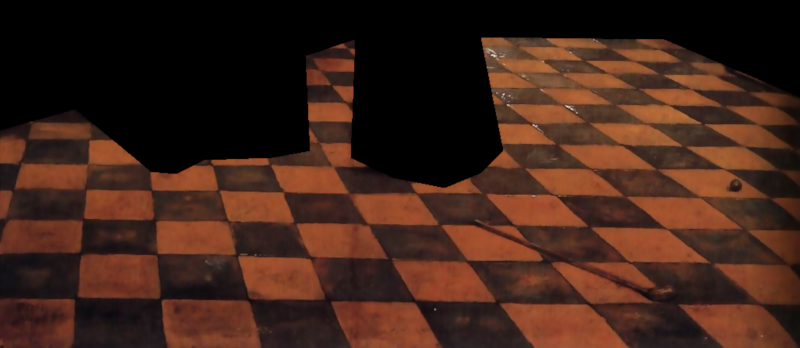
\includegraphics[scale=1.125]{bilateral2.png}};
		\node at (8.15, 0) {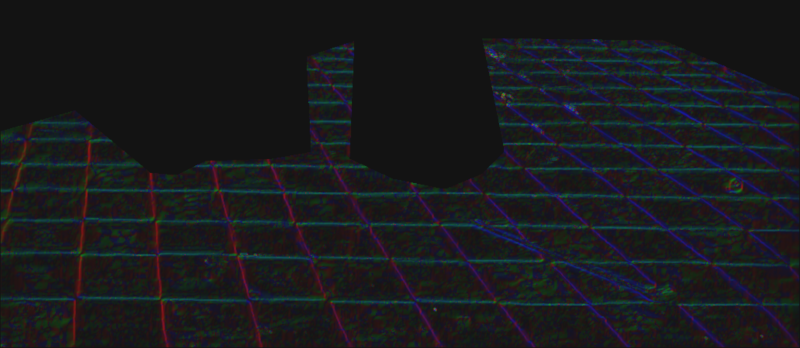
\includegraphics[scale=1.125]{sobel0.png}};
		\end{tikzpicture}
		\vspace{-4mm}
		\caption{Result of the Sobel filter}
		\label{im:sob}
	\end{figure}
	\vspace{-2mm}

	\paragraph{}
	In the \figurename \ref{im:sob} we can see the result obtained on the same painting used in the previous part about smoothing (I will use this painting throughout the explanation of the algorithm). The image on the left is the smoothed paint from the previous part and the one on the right is the image representing the gradient. For each pixel, the intensity of the color represents the norm of the gradient. In the image I give, the intensity is proportional to the square root of the norm. This choice was made so that it could be seen that despite the smoothing done previously, the gradient norm is not zero inside the tiles. The color gives the angle of the gradient. Red for $0+\Z \pi$, green for $\pi / 3 + \Z \pi$ and blue for $2\pi / 3 + \Z \pi$.
	
	\paragraph{Automatic cleaning}
	To eliminate the remaining noise and make the rest easier, I clean the image a little bit. To do so, I apply a threshold that will zero all pixels in the gradient whose intensity is less than a certain value. Then I compute the connected components of the remaining pixels and zero all pixels of the connected components that have a size smaller than a minimum size. I have a function that calculates the intensity threshold and minimum size of the related components based on the characteristics of the image. Unfortunately, these two values are not always perfect. I therefore allow the user to modify these values if necessary using sliders. The effect of this cleaning is illustrated in \figurename \ref{im:clean}.
	
	\begin{figure}[h]
		\centering
		\begin{tikzpicture}
		\node (a) at (0, 0) {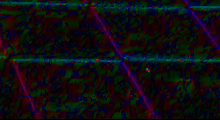
\includegraphics[scale=2.75]{sobel_wc.png}};
		\node (b) at (7, 0) {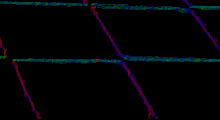
\includegraphics[scale=2.75]{sobel_c.png}};
		\draw[->, ultra thick] (a) -- node[above] {\small Cleaning} (b);
		\node (c) at (6.5, -1.98) {\footnotesize Erased because connected component too small};
		\draw[->, thick, gray] (c.174) -- (0.98, -0.35);
		\node (d) at (0, -1.72) {\footnotesize Erased because the intensity is too low};
		\draw[->, thick, gray] (d.north) -- (-0.85, -0.5);
		\end{tikzpicture}
		\vspace{-1mm}
		\caption{Cleaning the gradient image}
		\label{im:clean}
	\end{figure}

	\paragraph{Smoothing}
	It can be noted that the direction of the gradient is not perfect. Some isolated pixels, or even groups of pixels, do not have a good direction. However, in the following I will use this direction to find the lines. That's why I smooth the direction in the gradient image. The \textsc{Algorithm} \ref{alg:gsmooth} at the top of the next page is the function that gives the new smoothed value of a pixel of the gradient.
	
	\begin{algorithm}[h]
		\caption{Gradient Smoothing}
		\label{alg:gsmooth}
		\begin{algorithmic}
			\State $M \gets \begin{bmatrix}
				0.0925 & 0.12 & 0.0925 \\
				0.12 & 0.15 & 0.12 \\
				0.0925 & 0.12 & 0.0925
			\end{bmatrix}$
			\Function{SmoothGrad}{$G, \Theta, x, y$}
			\State $a, b \gets 0, 0$
			\For{$i, j \in \{ -1, 0, 1 \}^2$}
				\State $a \gets a + M[j+1][i+1] \times G[x+i][y+j] \times \cos \left( 2 \times \Theta[x+i][y+j] \right)$
				\State $b \gets b + M[j+1][i+1] \times G[x+i][y+j] \times \sin \left( 2 \times \Theta[x+i][y+j] \right)$
			\EndFor
			\State $\Theta[x][y] \gets \arg \left( a + ib \right) \, / \, 2$
			\EndFunction
		\end{algorithmic}
	\end{algorithm}

	The function computes a weighted average of the gradient angle $\Theta$ in a neighborhood of size $3 \times 3$ around the pixel $(x, y)$. The weight depends on the distance (thanks to the $M$ matrix) and the amplitude of the gradient ($G$). In addition, the factor 2 that appears in the cosine and sinus comes from the fact that we consider angles modulo $\pi$. Finally, because a single step of this smoothing is not enough, this algorithm is called several times. For example, for the paint that we use as an example, we apply 5 times the smoothing. For higher resolution images (because this one is low resolution), I can apply up to 15 smoothing steps for the gradient. The \figurename \ref{im:gsmooth} shows the result of the previous algorithm.
	
	\begin{figure}[h]
		\centering
		\begin{tikzpicture}
		\node[] (a) at (0, 0) {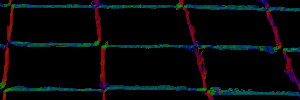
\includegraphics[scale=3.3]{sobel_ws.png}};
		\node[] (b) at (0, -3) {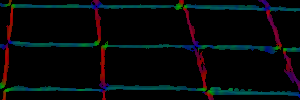
\includegraphics[scale=3.3]{sobel_s.png}};
		\node[below=3mm, white] at (a.150) {\small \, Without smoothing};
		\node[below=3mm, white] at (b.150) {\small With smoothing};
		\end{tikzpicture}
		\vspace{-1mm}
		\caption{Smoothing gradient result}
		\label{im:gsmooth}
	\end{figure}

	\paragraph{Manual cleaning} Because there may be objects on the floor of the paint or sometimes because the noise is too high (or because we can see some damages on the paints of high quality) there may be undesirable parts left in the gradient image. That's why I'm leaving user control again. There is the possibility of using a brush to remove unwanted parts. The user can choose the size of the brush and erase bad brush strokes that he could have given. The \figurename \ref{im:brush} illustrates this tool. White pixels are the erased gradient pixels.
	
	\begin{figure}[h]
		\centering
		\begin{tikzpicture}
		\node (a) at (0, 0) {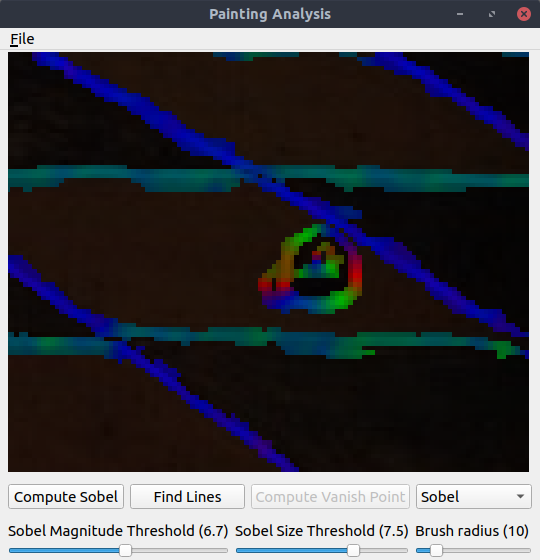
\includegraphics[scale=0.18]{w_man_c.png}};
		\node (b) at (6, 0) {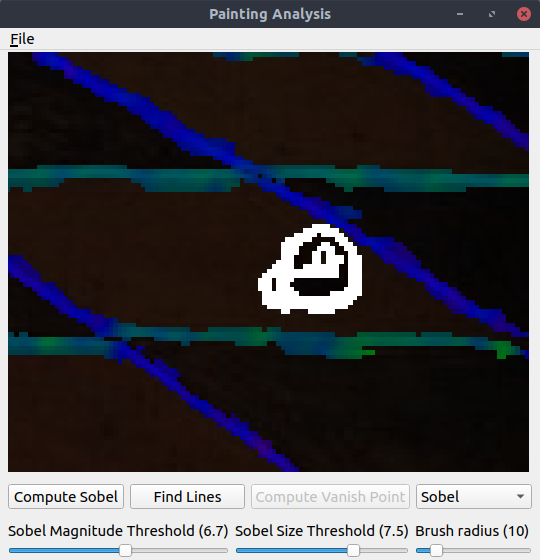
\includegraphics[scale=0.18]{man_c.png}};
		\draw[->, ultra thick] (a) -- node[above] {\small brush stroke} (b);
		\end{tikzpicture}
		\vspace{-2mm}
		\caption{Usage of the brush}
		\label{im:brush}
	\end{figure}
	
	\subsection{Hough Transform}
	
	\paragraph{A first try}
	Before using Hough's transform I tried something else that I will describe in a few lines in this paragraph. We are trying to find the main lines that make up the image. My idea was to compute connected components on the pixels of the gradient. I considered two pixels, adjacent if they touched each other and if their gradient angle difference was less than a certain value. Then I performed a PCA (Principal Component Analysis) \cite{pca} on each connected component in order to obtain equations of lines corresponding to the main direction of each component. Then I merged all the related components for which the guide lines were close and re-performed a PCA again to obtain new, more precise line equations.
	
	\paragraph{}
	But the big problem is that the principal component analysis was not very good on the small connected components and some lines were mainly formed by a succession of small connected components especially in paintings with very small tiles. Then there is a butterfly effect, some components merge when they should not, and others do not merge when they should. The results were therefore not very good and I implemented the Hough transform \cite{hough} which gave much better results.
	
	\paragraph{Parametrization}
	We often represent a line with two parameters $a$ and $b$, by the equation:
	\vspace{-2.2mm} $$ y = ax + b \vspace{-2.2mm} $$ 
	But this representation has some drawbacks. The parameters are not bounded if we consider all the lines passing through a rectangle. Fortunately, Duda and Hart have designed another representation that allows us to have bounded parameters $\rho$ and $\theta$:
	\vspace{-2.2mm} $$ \rho = x \cos(\theta) + y \sin(\theta) \vspace{-2.2mm} $$
	Thus $\rho$ represents the distance between the line and the origin except for the sign and $\theta$ represents the angle of the line normal. Let's call $D$ the length of the diagonal of the image. In the literature we generally take $\theta$ in $[0; \pi[$ and $\rho$ in $[-D; D]$. For my part, I preferred to take $\theta$ in $[-\pi / 2; \pi]$ and $\rho$ in $[0; D]$. These domains cover the entire rectangle of the image, \textit{i.e.} $[0; W) \times[0; H)$.
	
	\paragraph{Algorithm}
	The idea of the algorithm is to build a new image $H$, of size $R \times T$ where $R$ and $T$ are fixed using the dimensions of the original image. Then for each pixel of position $(x, y)$ of the gradient with a non-zero intensity, and for each $t \in[0; T)$ we compute the distance at the origin, $\rho$ of the line of direction $\theta = 3 \pi / 2 \times t / T - \pi / 2$ passing by $ (x, y)$. We then let $r = R * \rho / D$ and we add a positive value to the pixel of coordinates $(r, t)$ in the image $H$ (\textsc{Algorithm} \ref{alg:hough}).
	
	\begin{algorithm}[h]
		\caption{Hough Transform}
		\label{alg:hough}
		\begin{algorithmic}
			\Function{Hough}{$G, \Theta$}
			\State $H \gets $ Null image of size $R \times T$
			\For{$(x, y) \in [0, W) \times [0; H) $ with $ G[x][y] > 0$}
				\For{$t \in [0; T)$}
					\State $\theta \gets 3 \pi / 2 \times t / T - \pi / 2$
					\State $\rho \gets x . \cos(\theta) + y . \sin(\theta)$
					\If{$\rho \geqslant 0$}
						\State $r \gets \rho \times R / D$
						\State $H[r][t] \gets H[r][t] + f(G, \Theta, \theta, x, y)$
					\EndIf
				\EndFor
			\EndFor
			\State \Return $H$
			\EndFunction
		\end{algorithmic}
	\end{algorithm}

	\paragraph{}
	When Hough transform is computed, lines are local maximums of $H$. To obtain these local maximums, I sort all the pixels of the transform in descending order and then take the pixels one by one and add them to a list $L$ of lines if and only if the line corresponding to the pixel in question is far enough away from all the other lines already contained in the list $L$.
	
	\paragraph{}
	The value $H[r][t]$ then corresponds approximately to the number of pixels of the gradient on the line parameterized by $r$ and $t$. I say approximately because of the function $f$. This function allows you to take into account the intensity of the gradient and the difference between the angle of the line and the angle of the gradient. I have designed the following function:
	$$ f(G, \Theta, \theta, x, y) = \left( 1 - \left| \sin \left( \theta - \Theta[x][y] \right) \right|^{\frac{2}{3}}\right) \times \left( 1 + \frac{3}{2} \dfrac{G[x][y]}{\max (G)} \right) $$
	
	\begin{figure}[h]
		\centering
		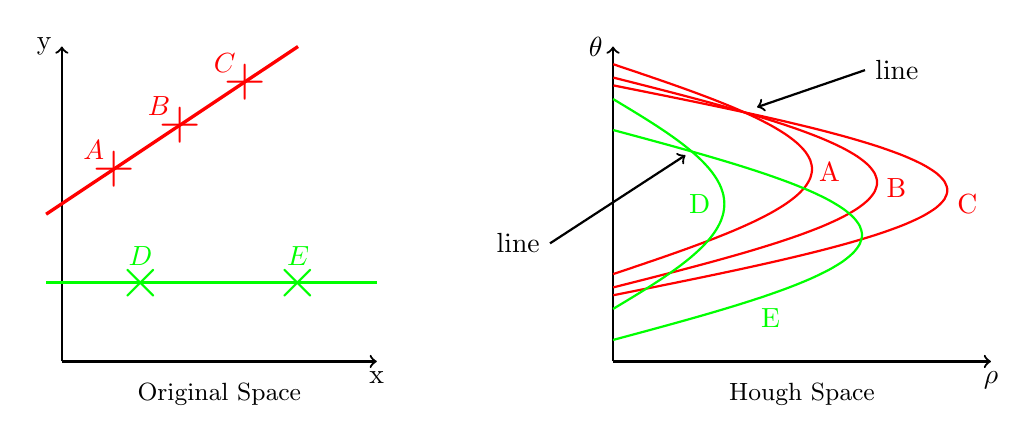
\begin{tikzpicture}
		\draw[->, thick] (0, 0) -- (4, 0) node[below] {x};
		\draw[->, thick] (0, 0) -- (0, 4) node[left] {y};
		\draw[very thick, red] (-0.2, 1.87) -- (3, 4);
		\node[red] (a) at (0.66, 2.44) {\huge $+$};
		\node[red] (b) at (1.5, 3) {\huge $+$};
		\node[red] (c) at (2.33, 3.55) {\huge $+$};
		\node[above left, red] at (a) {$A$};
		\node[above left, red] at (b) {$B$};
		\node[above left, red] at (c) {$C$};
		\draw[very thick, green] (-0.2, 1) -- (4, 1);
		\node[green] (a) at (1, 1) {\huge $\times$};
		\node[green] (b) at (3, 1) {\huge $\times$};
		\node[above=1mm, green] at (a) {$D$};
		\node[above=1mm, green] at (b) {$E$};
		
		\draw[->, thick] (7, 0) -- (11.8, 0) node[below] {$\rho$};
		\draw[->, thick] (7, 0) -- (7, 4) node[left] {$\theta$};
		\draw[variable=\t, domain=-0.264:2.877, smooth, thick, red]
			plot({7 + 0.66 * cos(\t*180/3.142) + 2.44 * sin(\t*180/3.142)}, {(\t + 1.571) / 4.713 * 4});
		\draw[variable=\t, domain=-0.463:2.677, smooth, thick, red]
			plot({7 + 1.5 * cos(\t*180/3.142) + 3 * sin(\t*180/3.142)}, {(\t + 1.571) / 4.713 * 4});
		\draw[variable=\t, domain=-0.580:2.560, smooth, thick, red]
			plot({7 + 2.33 * cos(\t*180/3.142) + 3.55 * sin(\t*180/3.142)}, {(\t + 1.571) / 4.713 * 4});
		\node[red] at (9.75, 2.4) {A};
		\node[red] at (10.6, 2.2) {B};
		\node[red] at (11.5, 2) {C};
		\draw[variable=\t, domain=-0.785:2.356, smooth, thick, green]
			plot({7 + 1 * cos(\t*180/3.142) + 1 * sin(\t*180/3.142)}, {(\t + 1.571) / 4.713 * 4});
		\draw[variable=\t, domain=-1.249:1.892, smooth, thick, green]
			plot({7 + 3 * cos(\t*180/3.142) + 1 * sin(\t*180/3.142)}, {(\t + 1.571) / 4.713 * 4});
		\node[green] at (8.1, 2) {D};
		\node[green] at (9, 0.55) {E};
		
		\draw[->, thick] (6.2, 1.5) node[left] {line} -- (7.92, 2.62);
		\draw[->, thick] (10.2, 3.7) node[right] {line} -- (8.83, 3.23);
		\node at (2, -0.42) {\small Original Space};
		\node at (9.4, -0.42) {\small Hough Space};
		\end{tikzpicture}
		\vspace{-1mm}
		\caption{Hough Transform Example}
		\label{im:houghe}
	\end{figure}

	The \figurename \ref{im:houghe} shows the curves where the Hough transform is strictly positive for five points sampled on two lines. The local maximums are located where the curves intersect. The two intersection points observed therefore correspond to the two lines that were sampled.
	
	\paragraph{Improvements}
	This algorithm can be improved in many ways to reduce the computation time but also to improve the final result. Here are the main improvements I have implemented:
	\begin{itemize}
		\item We don't have to go through the whole spectrum of $\theta$ but just limit ourselves to a smaller window around $\Theta[x][y]$. This limits the computation time and prevents some pixels from contributing to a line that does not correspond at all to the orientation of the gradient.
		\item After computing $\rho$ for a given pixel and direction $\theta$, instead of taking $r$ as a rounding of $\rho \times R/D$ we can take the two integers $r_1 = \lfloor \rho \times R/D \rfloor$ and $r_2 = \lceil \rho \times R/D \rceil$ and add a portion from $f(G, \Theta, \theta, x, y)$ to $H[r_1][t]$ and $H[r_2][t]$.
		\item The values $H[r][t]$ can be readjusted according to the distance that the line parameterized by $r$ and $t$ travels in the cut area of the image (see \figurename \ref{im:cut}).
		\item Once you have found that the pixel $(r, t)$ of the Hough transform corresponds to a local maximum and therefore to a line, you can use the values of the Hough transform in a small neighbourhood of $(r, t)$ to readjust the parameters $\rho$ and $\theta$ of the corresponding line.
	\end{itemize}
	
	\begin{figure}[h]
		\centering
		\begin{tikzpicture}
		\node (a) at (0, 0) {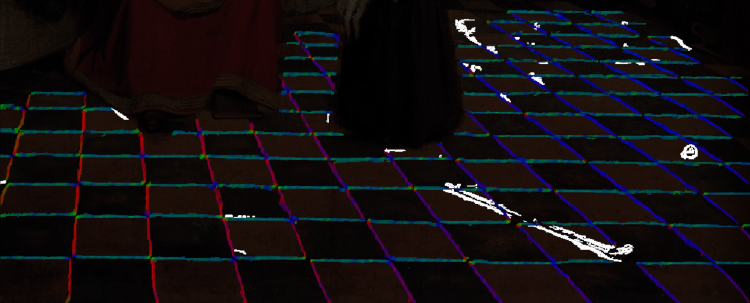
\includegraphics[scale=1.15]{sobel_final.png}};
		\node (b) at (8.3, 0) {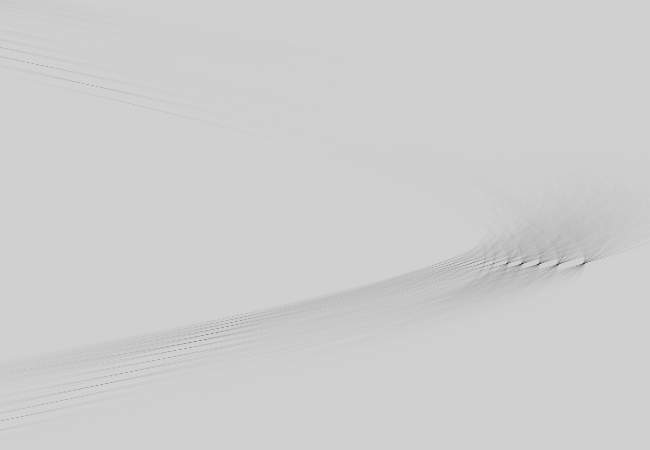
\includegraphics[scale=1.15]{hough_painting.png}};
		\draw[->, ultra thick] (a) -- node[above, align=center] {\small Hough \\[-1mm] \small trans.} (b);
		\node at (4.15, -6.25) {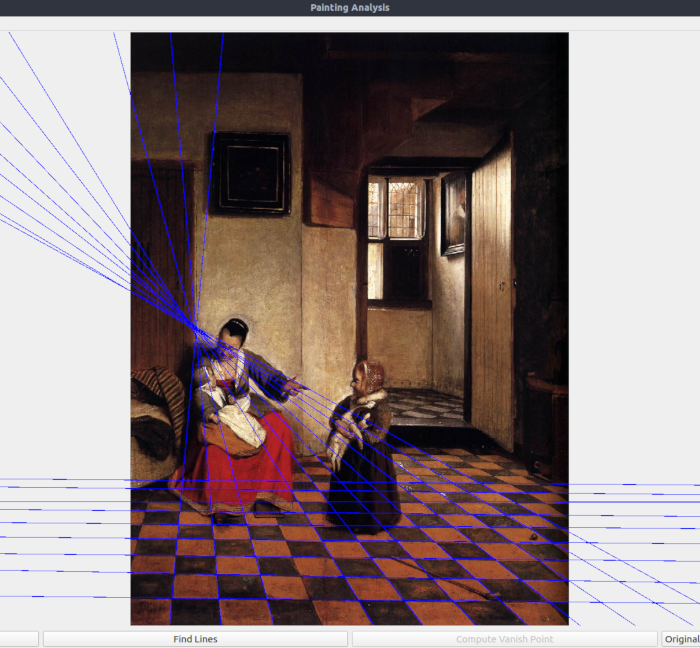
\includegraphics[scale=1.32]{lines0.png}};
		
		\draw[->, thin, red] (10.8, -0.42) -- (7.8, -9.34);
		\draw[->, thin, red] (10.555, -0.416) -- (7.33, -9.12);
		\draw[->, thin, red] (10.04, -0.417) -- (7.15, -8.5);
		\draw[->, thin, red] (5.95, 1.34) -- (2.8, -3.2);
		\draw[->, thin, red] (6.06, -1.598) -- (1.35, -4.6);
		\end{tikzpicture}
		\caption{Hough Transform on painting}
		\label{im:hough}
	\end{figure}

	\paragraph{}
	On the \figurename \ref{im:hough} we can see what the transform gives on the painting we have been following since the beginning. Only the 20 best lines are displayed in the interface after clicking on the button to find the lines. But the user has the possibility to delete the lines that do not interest him with the right click and to add the lines that the Hough transform found without them being displayed by right-clicking approximately where the desired line should be. The user also has the possibility to drag the mouse to indicate approximately the direction of the line if the position of the click is not really accurate. As mentioned in the subsection \ref{s:general}, the user can then group the lines together to compute the vanishing points (they are computed by minimizing the average square distances with the group lines) and also to compute the diagonals of the tiles. Diagonals are calculated by applying a PCA \cite{pca} to the intersections of the horizontal and depth lines. Finally, it is possible to save the result obtained in SVG format. The \figurename \ref{im:final} shows the result obtained for the painting we are following. It can then be seen that even if the vanishing line is not very horizontal, the perspective seems to be respected since the parallel lines all intersect well at the same point and all these vanishing points are approximately on the same line.
	
	\begin{figure}[h]
		\centering
		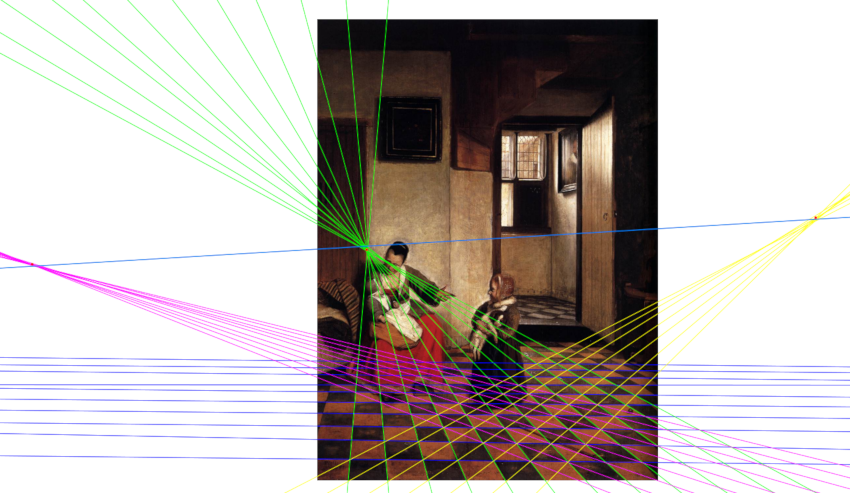
\includegraphics[scale=2]{final.png}
		\caption{Final Result}
		\label{im:final}
	\end{figure}

	\paragraph{}
	Results on different paintings are given in the appendices. I also give for some of them the difference obtained between the lines drawn by my algorithm and the lines drawn by Ricardo.	Finally, we would also like to know how close or far away the painting is to a perfect perspective. Indeed, we would like to know if it is possible that the artist made small inaccuracies or if he did not completely take into account the rules of perspective. Moreover, my algorithm is not necessarily very precise and therefore it can be interesting to see that a perfect perspective can be very close to the painting. This is the purpose of the next section. 

	\section{Attempt to redraw the paintings with a perfect perspective}
	
	\paragraph{}
	Elmar suggested I use the paper \textit{Structure preserving manipulation of photographs} \cite{redraw} that allows us to modify an image by using the its gradient. The idea is then to do the following steps starting from the lines obtained in the previous section:
	\begin{itemize}
		\item Compute new lines for the tiles that would all intersect exactly at a single vanishing point and remain as close as possible to the previously obtained lines.
		\item Modify the gradient of the image so that the high intensity pixels are on the new lines.
		\item Use Poisson editing \cite{poisson} to obtain the new image with perfect perspective from the new gradient.
	\end{itemize}
	Unfortunately, I didn't get anything conclusive for this second step. I will therefore only describe what I was able to do for the first step.
	
	\paragraph{}
	For the first step I parametrize the perspective with the coordinates of the points $A$, $B$ and $C$ and with the distances $d_A$, $d_B$ and $d_C$ (see \figurename \ref{im:tiledfloor}) between the intersections of the paintings lines with a line parallel to the vanishing line and located at a distance $d_{trans}$ from it. Thanks to the equations \eqref{eq:B} and \eqref{eq:dB} we can remove $B$ and $d_B$ from our parametrization. We then have 6 parameters to optimize:
	\vspace{-1mm} $$ x_A, \, y_A, \, x_C, \, y_C, \, d_A, \, d_C \vspace{-1mm} $$
	I have broken down the function that these parameters should minimize into the sum of three sub-functions explained in the next paragraphs. In the following I will use $c^{te}$ to designate a constant whose value won't be given in order not to overload the expression with uninteresting details. And I will also use $v$ to designate an expression that does not depend on the parameters to be minimized but that is dependent on the lines of the painting to which we are trying to be the closest.
	
	\paragraph{}
	In order to have a horizontal vanishing line and in order to have well oriented tiles, I try to minimize the following value:
	\begin{equation}
		\label{eq:R}
		R = \dfrac{(y_C - y_A)^2}{(x_C - x_A)^2 + (y_C - y_A)2} \times \left( v . (d_C - d_A)^2 + c^{te} \right)
	\end{equation}
	The left-side of the multiplication is null when the vanishing line is horizontal and strictly positive otherwise. The right-side try to minimize the difference between $d_C$ and $d_A$ because if these two values are equal then tiles are correctly oriented.
	
	\paragraph{}
	So that the vanishing points do not diverge too much, I minimize also this expression:
	\begin{equation}
		\label{eq:S}
		S = v . (x_A - x_{A_0})^2 + v . (y_A - y_{A_0})^2 + v . (x_B - x_{B_0})^2 + v . (y_B - y_{B_0})^2 + v . (x_C - x_{C_0})^2 + v . (y_C - y_{C_0})^2
	\end{equation}
	Where $B$ and $d_B$ are still given by the equations \eqref{eq:B} and \eqref{eq:dB}. The points $A_0$, $B_0$ and $C_0$ are the vanishing points obtained in the previous section, the ones that are represented by red dots in the \figurename \ref{im:final}. This expression $S$ is simply the sum of the square distances of the new vanishing points to the old ones.
	
	\paragraph{}
	The last expression to minimize is the most complicated one. With the two previous expressions $R$ and $S$ we only take care of the vanishing line and the vanishing points but we don't take care of the position of the lines in the paintings. In order not to have something too complicated to optimize, I decided to make sure that for each group of parallel lines, the endpoints of the right-most line and the left-most line match as closely as possible with the endpoints of initial lines.
	
	\begin{figure}[h]
		\centering
		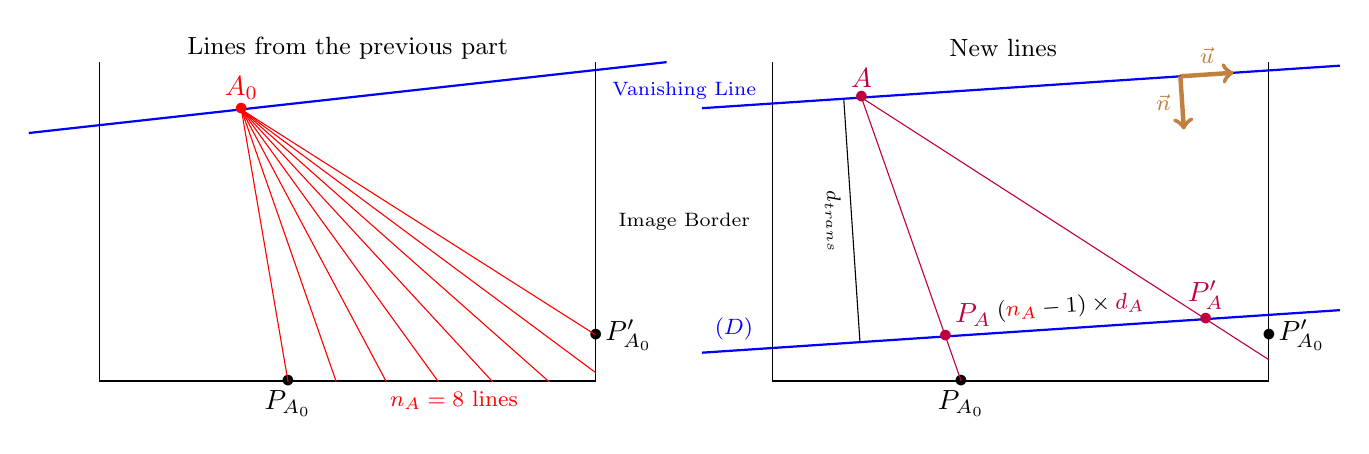
\begin{tikzpicture}[scale=0.9]
			\node at (1.5, 4.7) {\small Lines from the previous part};
			\draw (-2, 4.5) -- (-2, 0) -- (5, 0) -- (5, 4.5);
			\draw[blue, thick] (-3, 3.5) -- (6, 4.5) ;
			\node[red] at (0, 3.83) {$\bullet$};
			\node[red, above] at (0, 3.83) {$A_0$};
			\node at (0.657, 0) {$\bullet$};
			\node[below] at (0.657, 0) {$P_{A_0}$};
			\node at (5, 0.651) {$\bullet$};
			\node[right] at (5, 0.651) {$P'_{A_0}$};
			\node[red, below] at (3, 0) {\footnotesize $n_A = 8 \text{ lines}$};
					
			\begin{scope}
			\clip (-2, 4.5) rectangle (5, 0);
			\foreach \i in {0, ..., 7} \draw[red] (0, 3.83) -- ({0.994*\i + 1}, {0.11*\i - 2});
			\end{scope}
			
			\node[blue] at (6.25, 4.1) {\scriptsize Vanishing Line};
			\node[] at (6.25, 2.25) {\scriptsize Image Border};
			
			\node at (10.75, 4.7) {\small New lines};
			\draw (7.5, 4.5) -- (7.5, 0) -- (14.5, 0) -- (14.5, 4.5);
			\draw[blue, thick] (6.5, 3.85) -- (15.5, 4.45);
			\draw[blue, thick] (6.5, 0.4) --
				node[pos=0.05, above] {\footnotesize $(D)$}
				node[pos=0.58, sloped, above] {\footnotesize
					$\color{black} ({\color{red} n_A} - 1) \times {\color{purple} d_A}$}
				(15.5, 1);
			\draw (8.5, 3.983) -- node[left, below, sloped] {\scriptsize $d_{trans}$} (8.729, 0.549);
			\node[purple] at (8.75, 4) {$\bullet$};
			\node[purple, above] at (8.75, 4) {$A$};
			\node at (10.157, 0) {$\bullet$};
			\node[below] at (10.157, 0) {$P_{A_0}$};
			\node at (14.5, 0.651) {$\bullet$};
			\node[right] at (14.5, 0.651) {$P'_{A_0}$};
			
			\node[purple] at (9.936, 0.629) {$\bullet$};
			\node[purple, above right] at (9.936, 0.629) {$P_A$};
			\node[purple] at (13.608, 0.874) {$\bullet$};
			\node[purple, above] at (13.608, 0.874) {$P'_A$};
			
			\draw[ultra thick, brown, ->] (13.25, 4.3) -- node[above] {\footnotesize $\vec{u}$} (14, 4.35);
			\draw[ultra thick, brown, ->] (13.25, 4.3) -- node[left] {\footnotesize $\vec{n}$} (13.3, 3.55);
			
			\draw[purple] (8.75, 4) -- (10.157, 0);
			\draw[purple] (8.75, 4) -- (14.5, 0.3);
		\end{tikzpicture}
		\vspace{-5mm}
		\caption{Constructions of a few points for the function to be minimized}
		\label{im:cons}
	\end{figure}

	We call $P_{A_0}$ the endpoint of the left-most line whose vanishing point is $A_0$ and $P'_{A_0}$ the endpoint of the right-most line whose vanishing point is also $A_0$. We define $P_{B_0}$, $P'_{B_0}$, $P_{C_0}$ and $P'_{C_0}$ in the same way. Here I will only explain what I minimize for the lines whose vanishing points is $A$, but you can replace $A$ with $B$ or $C$ for the rest of the paragraph. We can also define the unit vanishing line direction vector $\vec{u} \,$ by the normalization of $\overrightarrow{AC}$. Then we can obtain the normal unit vector $\vec{n} \,$ by a simple rotation of minus 90 degrees. Now our goal is to compute the distance between $P'_{A_0}$ and the new right-most line assuming that the left-most line passes through $P_{A_0}$. To do this, we use the fact that the intersections of lines whose vanishing point is $A$ with the line $(D)$ (the one parallel to the vanishing line and located at a distance $d_{trans}$ from it) are spaced from the distance $d_A$. Thus we define $P_A$ as the intersection between $(D)$ and $(A P_{A_0})$:
	$$ P_A = A + d_{trans} \, / \, \left( \vec{n} . \overrightarrow{A P_{A_0}} \right) \times \overrightarrow{A P_{A_0}} $$
	Therefore the right-most line passes through the point $P'_A$ defined by:
	$$ P'_A = P_A + (n_A - 1) \times d_A \times \vec{u} $$
	Where $n_A$ is the number of lines whose vanishing points is $A$. We finally get the wanted distance:
	$$ dist \left( (A P'_A), \, P'_{A_0} \right) = \left| \det \begin{bmatrix} \overrightarrow{P'_A P'_{A_0}} & \overrightarrow{A P'_A} \end{bmatrix} \right| \; / \; \left\| \overrightarrow{A P'_A} \right\| $$
	The last term that we need to minimize is then:
	\begin{equation}
		\label{eq:T}
		T = dist \left( (A P'_A), \, P'_{A_0} \right)^2 + dist \left( (B P'_B), \, P'_{B_0} \right)^2 + dist \left( (C P'_C), \, P'_{C_0} \right)^2
	\end{equation}
	
	\paragraph{}
	Thanks to the equation \eqref{eq:R}, \eqref{eq:S} and \eqref{eq:T} we obtain the function to minimize:
	$$ F(x_A, y_A, x_C, y_C, d_A, d_C) = c^{te} . R \, + \, v . S \, + \, v . T $$
	This minimization is done using the Newton Raphson's method. With my way of initializing variables (which I will not detail) it generally takes no more than 3 steps of this method to converge.
	
	\begin{wrapfigure}{r}{2.9cm}
		\centering
		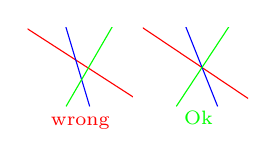
\begin{tikzpicture}[scale=1.25]
		\begin{scope}
		\clip (0.33, 0.8) rectangle (1.4, 0);
		\draw[red] (0, 1) -- (1.55, 0);
		\draw[blue] (0.66, 1) -- (0.96, 0);
		\draw[green] (1.3, 1) -- (0.72, 0);
		\end{scope}
		\node[red] at (0.865, -0.17) {\scriptsize wrong};
		
		\begin{scope}
		\clip (1.5, 0.8) rectangle (2.57, 0);
		\draw[red] (1.2, 1) -- (2.69, 0);
		\draw[blue] (1.86, 1) -- (2.26, 0);
		\draw[green] (2.5, 1) -- (1.84, 0);
		\end{scope}
		\node[green] at (2.065, -0.12) {\scriptsize Ok};
		\end{tikzpicture}
		\vspace{-5mm}
	\end{wrapfigure}
	Once the six parameters have been optimized, we actually obtain lines that remain close to the initial lines. But there is one thing wrong with it. Lines from the vanishing points $A$, $B$ and $C$ do not all intersect at the same time. There is a slight difference between the intersections of these lines two by two. I then slightly shift each group of lines along the direction of the vanishing line to ensure that the three groups intersect at the same time. Once this problem is solved, we obtain the result in the \figurename \ref{im:perf}
	
	\begin{figure}[h]
		\centering
		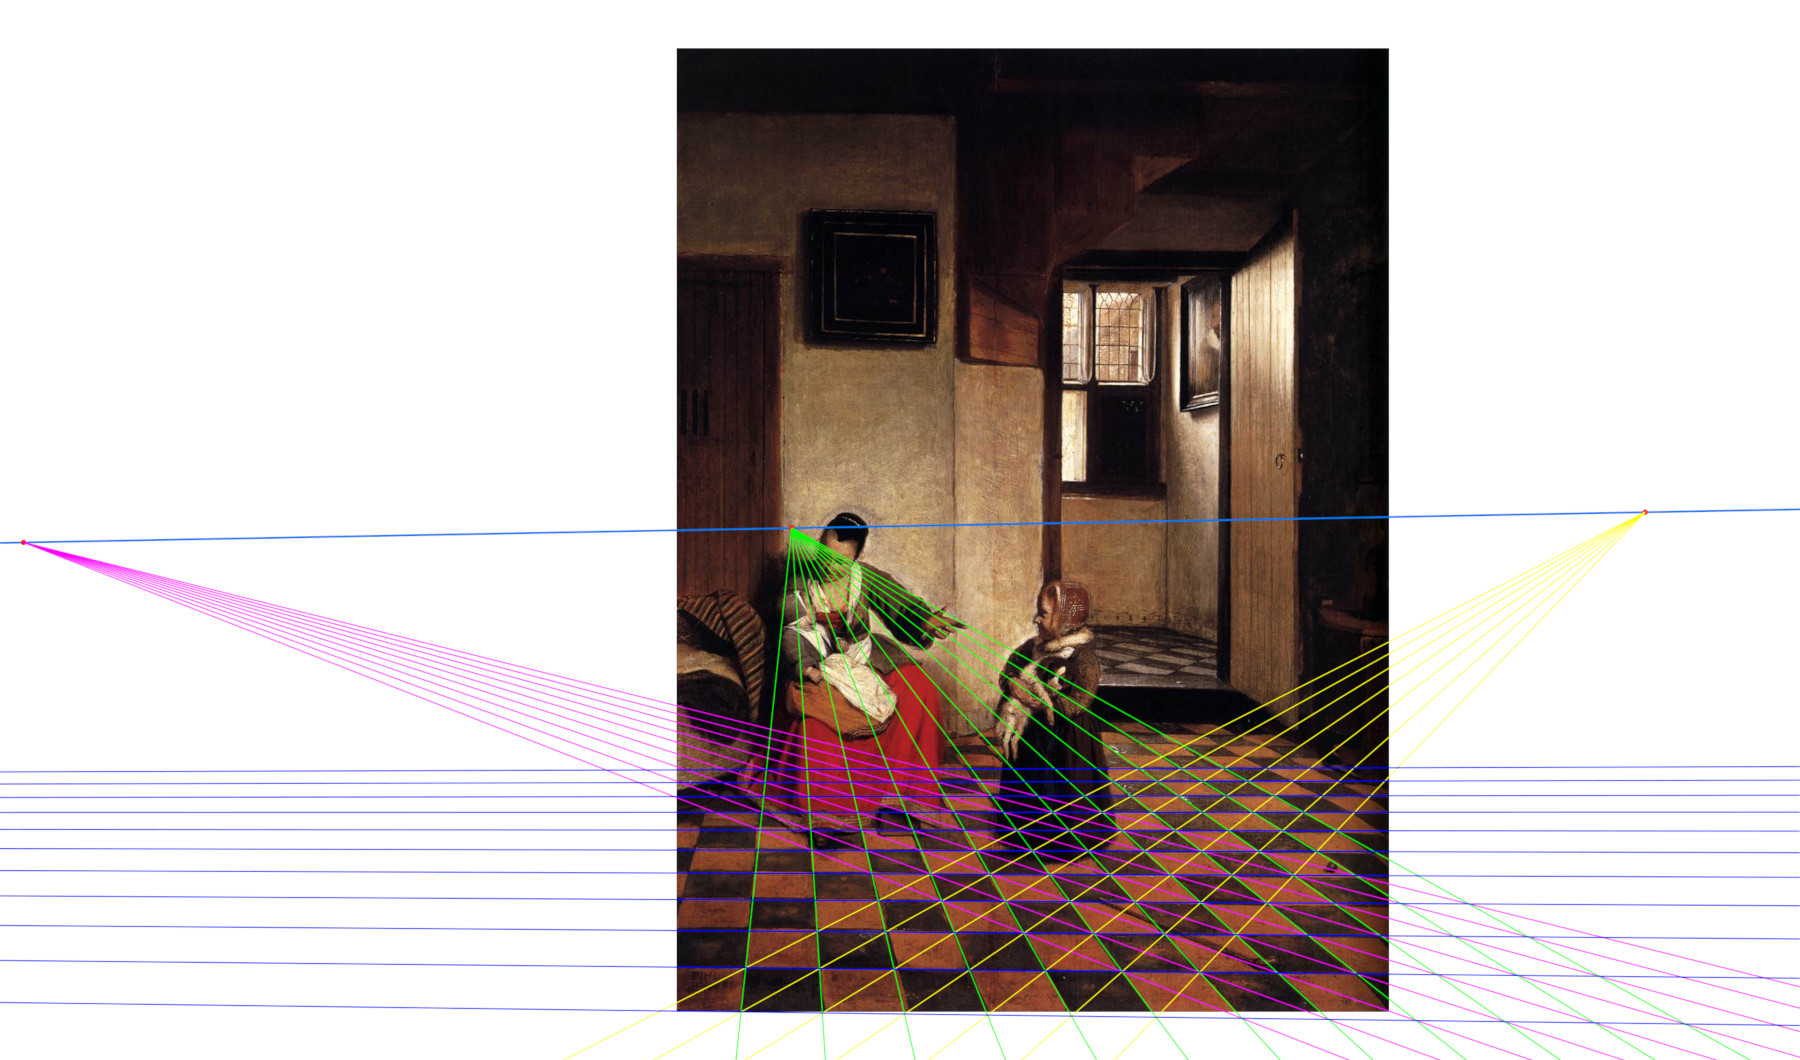
\includegraphics[scale=0.28]{perf.jpg}
		\vspace{-2mm}
		\caption{Result of the perfect perspective}
		\label{im:perf}
	\end{figure}

	\section{Conclusion}
	
	\appendix
	
	\section{Source Code}
	
	Here is my git repository: \url{https://github.com/Nanored4498/Painting-Analysis}.

	\bibliographystyle{alpha}
	\bibliography{bib.bib}
	
\end{document}